%\begin{document}

\begin{comment}
As a static language, much of the complexity in the implementation of \CEU{} 
resides in the compile phase.
Nonetheless, some complexity is left to the runtime phase, which has to manage 
first-class timers, finalization blocks, and all bookkeeping related to trails.
\end{comment}

The compilation process of a program in \CEU is composed of three main phases, 
as illustrated in Figure~\ref{fig.impl}:

\begin{figure}[ht]
\centering
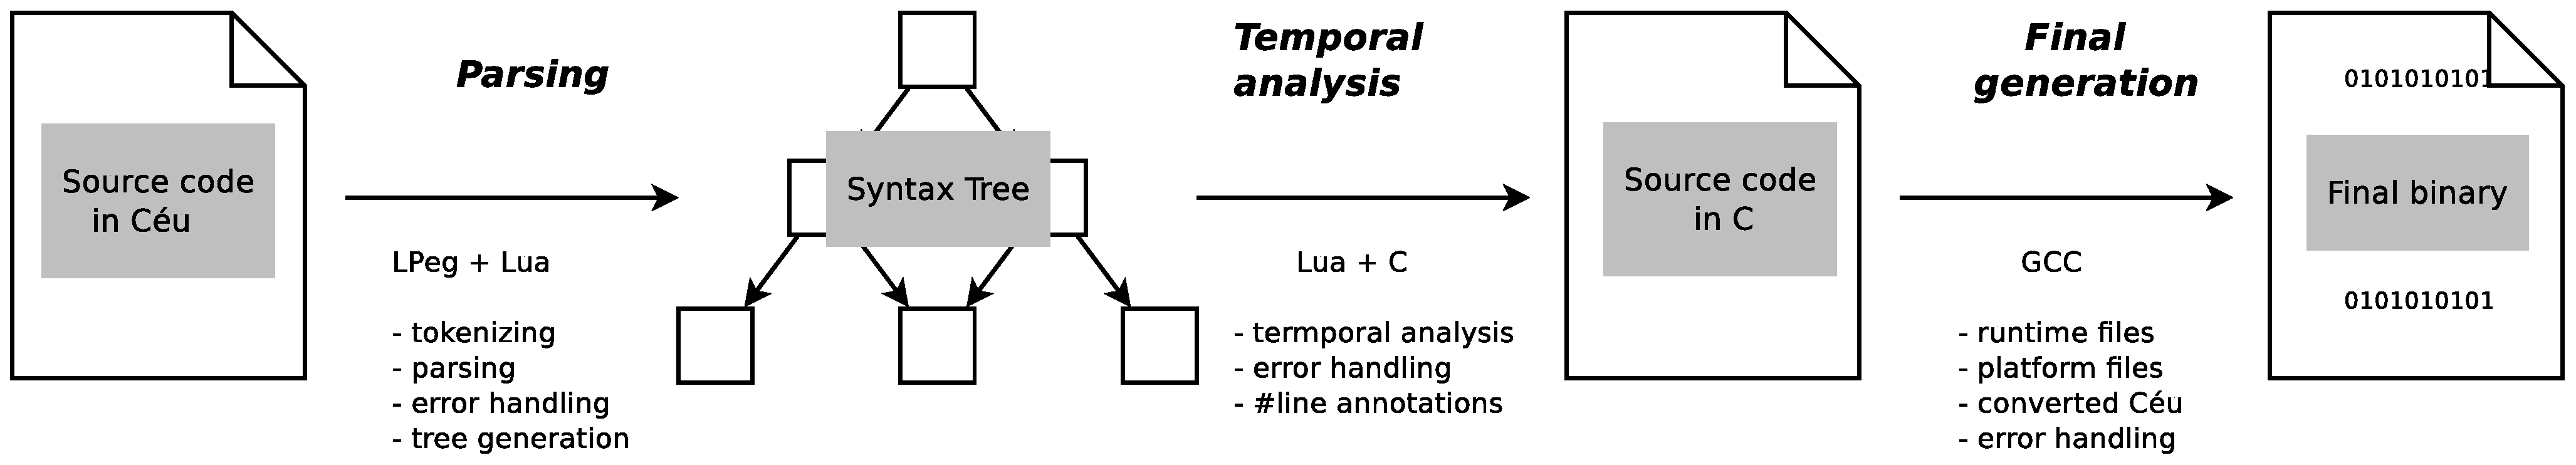
\includegraphics[scale=0.20]{impl}
\caption{ Compilation process: from the source code in \CEU to the final 
binary.
\label{fig.impl}
}
\end{figure}

\begin{comment}
The program below is used as our guiding example for this chapter:

\begin{lstlisting}[numbers=left,xleftmargin=2em]
input int A, B, C;
var int ret;
loop do
   par/or do
      do                            // 1st trail
          var int a = await A;
          ret = ret + a;
      end
      do
          var int b = await B;
          ret = ret + b;
      end
      break;
   with
      par/and do                    // 2nd trail
         finalize with
            ret = ret + 10;
         end
         await C;
      with
         await A;
      end
   end
end
...                                 // code after the loop
\end{lstlisting}
\end{comment}

\begin{description}

\item[Parsing]

The parser of \CEU is written in \emph{LPeg}~\cite{lua.lpeg}, a pattern 
matching library that also recognize grammars, making it possible to write the 
tokenizer and grammar with the same tool.
%
The source code is then converted to an \emph{abstract syntax tree (AST)} to be 
used in further phases.
%
This phase may be aborted due to syntax errors in the \CEU source file.

\item[Temporal analysis]

This phase detects inconsistencies in \CEU programs, such as unbounded loops 
and the forms of non-determinism.
%
It also makes some ``classical'' semantic analysis, such as building a symbol 
table for checking variable declarations.
However, most of type checking is delayed to the last phase to take advantage 
of GCC's error handling.
Therefore, this phase needs to annotate the $C$ output with \code{\#line} 
pragmas that match the original file in \CEU.
%
This phase must output code in $C$, given how tied \CEU is to $C$ by design.

\item[Final generation]

The final phase packs the generated $C$ file with the \CEU runtime and 
platform-dependent functionality, compiling them with \emph{gcc} and generating 
the final binary.
%
The \CEU runtime includes the scheduler, timer management, and the external $C$ 
API.
%
The platform files include libraries for I/O and bindings to invoke the \CEU 
scheduler on external events.

\end{description}

In the sections that follow, we discuss the most sensible parts of the compiler 
considering our design, such as the temporal analysis, runtime scheduler, and 
the external API.

\section{Temporal analysis}

As introduced, the \emph{temporal analysis} phase detects inconsistencies in 
\CEU programs.
Here, we focus on the algorithm that detects non-deterministic access to 
variables, as presented in Section~\ref{sec.ceu.shared}.

For each node representing a statement in the program AST, we keep the set of 
events $I$ (for \emph{incoming}) that can lead to the execution of the node, 
and also the set of events $O$ (for \emph{outgoing}) that can terminate the 
node.

A node inherits the set $I$ from its direct parent and calculates $O$ according 
to its type:
%
\begin{itemize}
%
\item Nodes that represent expressions, assignments, $C$ calls, and 
declarations simply reproduce $O=I$, as they do not await;
%
\item An \code{await e} statement has $O=\{e\}$.
%
\item A \code{break} statement has $O=\{\}$ as it escapes the innermost 
\code{loop} and never terminate (see also \code{loop} below);
%
\item A \emph{sequence node (;)} modifies each of its children to have 
$I_n=O_{n-1}$.
The first child inherits $I$ from the sequence parent, and the set $O$ for the 
sequence node is copied from its last child, i.e., $O=O_n$.
%
\item A \code{loop} node includes its body's $O$ on its own $I$ ($I=I \cup 
O_{body}$), as the loop is also reached from its own body.
The union of all \code{break} statements' $O$ forms the set $O$ for a 
\code{loop}.
%
\item An \code{if} node has $O=O_{true} \cup O_{false}$.
%
\item A parallel composition (\code{par/and} / \code{par/or}) may terminate 
from any of its branches, hence $O = O_1 \cup ... \cup O_n$.
\end{itemize}

With all sets calculated, any two nodes that perform side effects and are in 
parallel branches can have their $I$ sets compared for intersections.
If the intersection is not the empty set, they are marked as suspicious (see 
Section~\ref{sec.ceu.shared}).

Figure~\ref{lst.impl.ast} reproduces the second code of Figure~\ref{lst.det} 
and shows the corresponding $AST$ with the sets $I$ and $O$ for each node.
The event $.$ (dot) represents the ``boot'' reaction.
The assignments to \code{y} in parallel (lines 5,8 in the code) have an empty 
intersection of $I$ (lines 6,9 in the AST), hence, they do not conflict.
Note that although the accesses in lines 5, 11 in the code (lines 6,11 in the 
AST) do have an intersection, they are not in parallel and are also safe.

\begin{figure}[h]
\begin{minipage}[t]{0.45\linewidth}
\begin{lstlisting}
input void A, B;
var int y;
par/or do
  await A;
  y = 1;
with
  await B;
  y = 2;
end
await A;
y = 3;
\end{lstlisting}
\end{minipage}
%
%
\begin{minipage}[t]{0.55\linewidth}
\begin{lstlisting}[numbers=left,xleftmargin=2.5em]
Stmts I={.} O={A}
    Dcl_y I={.} O={.}
    ParOr I={.} O={A,B}
        Stmts I={.} O={A}
            Await_A I={.} O={A}
            Set_y I={A} O={A}
        Stmts I={.} O={B}
            Await_B I={.} O={B}
            Set_y I={B} O={B}
    Await_A I={A,B} O={A}
    Set_y I={A} O={A}
\end{lstlisting}
\end{minipage}
%
\rule{14cm}{0.37pt}
\caption{ A program with a corresponding AST describing the sets $I$ and $O$.
%{\small %\textmd{
The program is safe because accesses to \code{y} in parallel have no 
intersections for $I$.
%}%}
\label{lst.impl.ast}
}
\end{figure}


\begin{comment}
It is also responsible for setting the priorities for trails (see further) and 
determining the sizes of the queues that are used during runtime.

The program AST is first converted into a graph that represents the execution 
flow.
Figure~\ref{fig:nfa} shows the corresponding graph for our example.

\begin{figure}[ht]
\centering
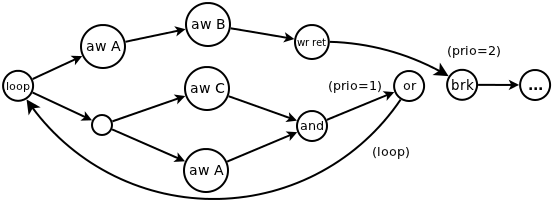
\includegraphics[scale=0.40]{nfa.png}
\caption{ Flow graph for our guiding example
\label{fig:nfa}
}
\end{figure}

By default, all nodes in a flow graph have priority $0$ (highest).
However, as the figure shows, nodes that represent the termination of 
\emph{par/ors} and loops have lower priorities (the outer, the lower).
The priority scheme is needed to avoid glitches during runtime, and is 
equivalent to traversing a dependency graph in topological order, as employed 
in functional reactive programming implementations.~\cite{frtime.embedding}

The flow graph is then converted to a DFA, as exemplified in 
Section~\ref{sec:ceu:det}.

From its starting node, the flow graph is traversed until reaching await 
nodes---every visited node is inserted into a new DFA state.
Then, every set of awaiting nodes for a given external event starts another DFA 
state.
\end{comment}

\section{Memory layout}
\label{sec:impl:memory}

\CEU{} favors a fine-grained use of trails, being common the use of trails that 
await a single event.
For this reason, \CEU{} does not allocate per-trail stacks; instead, all data 
resides in fixed memory slots---this is true for the program variables as well 
as for temporary values and flags needed during runtime.
%For instance, the first trail in the guiding example requires temporary slots 
%to hold the locals \code{a} and \code{b}, while the second trail must keep 
%flags to remember which sides of the \code{par/and} have already terminated.
%
Memory for trails in parallel must coexist, while statements in sequence can 
reuse it.
%In the example, the code following the loop (identified as \code{...}) reuses 
%all memory from the loop.
%
\CEU reserves a single static block of memory to hold all memory slots, whose 
size is the maximum the program uses at a given time.
A given position in the memory may hold different data (with variable sizes) 
during runtime.

\begin{figure}[t]
\begin{minipage}[t]{0.45\linewidth}
\begin{lstlisting}
input int A, B, C;
do
    var int a = await A;
end
do
    var int b = await B;
end
par/and do
    await B;
with
    await C;
end
\end{lstlisting}
\end{minipage}
%
\begin{minipage}[t]{0.55\linewidth}
\begin{lstlisting}
union {             // sequence
    int a_1;        //   do_1
    int b_2;        //   do_2
    struct {        //   par/and
        u8 _and_3: 1;
        u8 _and_4: 1;
    };
} MEM ;
\end{lstlisting}
\end{minipage}
\rule{14cm}{0.37pt}
\caption{
A program with blocks in sequence and in parallel, with corresponding memory 
layout.
{\small %\textmd{
}%}
\label{lst.impl.mem}
}
\end{figure}

Translating this idea to $C$ is straightforward~\cite{wsn.osm,wsn.ocram}: 
memory for blocks in sequence are packed in a \code{struct}, while blocks in 
parallel, in a \code{union}.
%
As an example, Figure~\ref{lst.impl.mem} shows a program with corresponding 
memory layout.
%
Each variable is assigned a unique $id$ (e.g. \code{a\_1}) so that variables 
with the same name can be distinguished.
%
The \code{do-end} blocks in sequence are packed in a \code{union}, given that 
their variables cannot be in scope at the same time, e.g., \code{MEM.a\_1} and 
\code{MEM.b\_2} can safely share the same memory address.
%
The example also illustrates the presence of runtime flags related to the 
parallel composition, which also reside in reusable slots in the static memory.

\section{Trail allocation}
\label{sec:impl:gates}

The compiler extracts the maximum number of trails a program can have at the 
same time and creates a static vector to hold runtime information about them.
Again, trails that cannot be active at the same time can share memory slots in 
the static vector.

At any given moment, a trail can be awaiting in one of the following states: 
\code{INACTIVE}, \code{STACKED}, \code{FIN}, or in any event defined in the 
program:

\begin{lstlisting}
enum {
    INACTIVE = 0,
    STACKED,
    FIN,
    EVT_A,      // input void A;
    EVT_e,      // event int e;
    <...>       // other events
}
\end{lstlisting}

All terminated or not-yet-started trails stay in the \code{INACTIVE} state and 
are ignored by the scheduler.
%
A \code{STACKED} trail holds its associated stack level and is delayed until 
the scheduler runtime level reaches that value again.
%
A \code{FIN} trail represents a hanged finalization block which is only 
scheduled when its corresponding block goes out of scope.
%
A trail waiting for an event stays in the state of the corresponding event, 
also holding the sequence number (\emph{seqno}) in which it started awaiting.
%
A trail is represented by the following \code{struct}:

\begin{lstlisting}
struct trail_t {
    state_t evt;
    label_t lbl;
    union {
        unsigned char seqno;
        stack_t       stk;
    };
};
\end{lstlisting}

The field \code{evt} holds the state of the trail (or the event it is 
awaiting); the field \code{lbl} holds the entry point in the code to execute 
when the trail is scheduled; the third field depends on the \code{evt} field 
and may hold the \code{seqno} for an event, or the stack level \code{stk} for a
\code{STACKED} state.

The size of \code{state\_t} depends on the number of events in the application;
for an application with less than 253 events (plus the 3 states), one byte is 
enough.
%
The size of \code{label\_t} depends primarily on the number of \code{await} 
statements in the application---each \code{await} splits the code in two and 
requires a unique entry point in the code for its continuation.
Additionally, split \& join points for parallel compositions, \code{emit} 
continuations, and finalization blocks also require labels.
%
The \code{seqno} will eventually overflow during execution (every 256 
reactions).
However, given that the scheduler traverses all trails in each reaction, it can 
adjust them to properly handle overflows (actually 2 bits to hold the 
\code{seqno} would be already enough).
%
The stack size depends on the maximum depth of nested emissions and is bounded 
to the maximum number of trails, e.g., a trail emits an event that awakes 
another trail, which emits an event that awakes another trail, and so on---the 
last trail cannot awake any trail, because they will be all hanged in a 
\code{STACKED} state.
%
In WSNs applications, the size of \code{trail\_t} is typically only 3 bytes (1 
byte for each field).

\subsection{Code generation}

\begin{figure}[t]
\begin{minipage}[t]{0.55\linewidth}
\begin{lstlisting}[numbers=left,xleftmargin=2em]
input void A;
event void e;
// TRAIL 0 - lbl Main
par/and do
  // TRAIL 0 - lbl Main
  await e;
  // TRAIL 0 - lbl Awake_e
  // TRAIL 0 - lbl ParAnd_chk
with
  // TRAIL 1 - lbl ParAnd_sub_2
  await A;
  // TRAIL 1 - lbl Awake_A_1
  emit e;
  // TRAIL 1 - lbl Emit_e_cont
  // TRAIL 1 - lbl ParAnd_chk
end
// TRAIL 0 - lbl ParAnd_out
await A;
// TRAIL 0 - lbl Awake_A_2
\end{lstlisting}
\end{minipage}
%
\begin{minipage}[t]{0.45\linewidth}
\begin{lstlisting}
enum {
  Main = 1,     // ln  3
  Awake_e,      // ln  7
  ParAnd_chk,   // ln  8, 15
  ParAnd_sub_2, // ln 10
  Awake_A_1,    // ln 12
  Emit_e_cont,  // ln 14
  ParAnd_out,   // ln 17
  Awake_A_2     // ln 19
};
\end{lstlisting}
\end{minipage}
\rule{14cm}{0.37pt}
\caption{
%{\small %\textmd{
Static allocation of trails and entry-point labels.
%}%}
\label{lst.impl.trails}
}
\end{figure}

The example in Figure~\ref{lst.impl.trails} illustrates how trails and labels 
are statically allocated in a program.
%
The program has a maximum of 2 trails, because the \code{par/and} (line 4) can 
reuse \emph{TRAIL 0}, and the join point (line 16) can reuse both \emph{TRAIL 
0} and \emph{TRAIL 1}.
%
Each label is associated with a unique identifier in the \code{enum}.
%
The static vector to hold the two trails in the example is defined as

\begin{lstlisting}
trail_t TRLS[2];
\end{lstlisting}

In the final generated $C$ code, each label becomes a \emph{switch case} 
working as the entry point to execute its associated code.
%
Figure~\ref{lst.impl.code} shows the corresponding code for the program of 
Figure~\ref{lst.impl.trails}.
%
The program is initialized with all trails set to \code{INACTIVE}.
Then, the scheduler executes the \emph{Main} label in the first trail.
%
When the \emph{Main} label reaches the \code{par/and}, it ``stacks'' the 2nd 
trail of the \code{par/and} to run on \emph{TRAIL 1} (line 5-8) and proceeds to 
the code in the 1st trail (lines 10-15), respecting the deterministic execution 
order.
%
The code sets the running \emph{TRAIL 0} to await \code{EVT\_e} on label 
\code{Awake\_e}, and then halts with a \code{break}.
%
The next iteration of the scheduler takes \emph{TRAIL 1} and executes its 
registered label \code{ParAnd\_sub\_2} (lines 17-22), which sets \emph{TRAIL 1} 
to await \code{EVT\_A} and also halts.


\begin{figure}[t]
\begin{lstlisting}[numbers=left,xleftmargin=2em]
while (<...>) {             // scheduler main loop
   trail_t* trail = <...>   // choose next trail
   switch (trail->lbl) {
      case Main:
         // activate TRAIL 1 to run next
         TRLS[1].evt = STACKED;
         TRLS[1].lbl = ParAnd_sub_2;  // 2nd trail of par/and
         TRLS[1].stk = current_stack;

         // code in the 1st trail of par/and
         // await e;
         TRLS[0].evt = EVT_e;
         TRLS[0].lbl = Awake_e;
         TRLS[0].seq = current_seqno;
         break;

      case ParAnd_sub_2:
         // await A;
         TRLS[1].evt = EVT_A;
         TRLS[1].lbl = Awake_A_1;
         TRLS[1].seq = current_seqno;
            break;

        <...>   // other labels
    }
}
\end{lstlisting}
\rule{14cm}{0.37pt}
\caption{
%{\small %\textmd{
Generated code for the program of Figure~\ref{lst.impl.trails}.
%}%}
\label{lst.impl.code}
}
\end{figure}

Regarding cancellation, trails in parallel are always allocated in subsequent 
slots in the static vector \code{TRLS}.
Therefore, when a \code{par/or} terminates, the scheduler sequentially searches 
and executes \code{FIN} trails within the range of the \code{par/or}, and then 
clears all of them to \code{INACTIVE} at once.
Given that finalization blocks cannot contain \code{await} statements, the 
whole process is guaranteed to terminate in bounded time.
Escaping a \code{loop} that contains parallel compositions also trigger the 
same process.

\section{The external $C$ API}

As a reactive language, the execution of a program in \CEU is guided entirely 
by the occurrence of external events.
From the implementation perspective, there are three external sources of input 
into programs, which are all exposed as functions in a $C$ API:

\begin{description}
\item[{\textbf\code{ceu\_go\_init()}}:] initializes the program (e.g. trails) 
and executes the ``boot'' reaction (i.e., the \code{Main} label).

\item[{\textbf\code{ceu\_go\_event(id,param)}}:] executes the reaction for the 
received event id and associated parameter.

\item[{\textbf\code{ceu\_go\_wclock(us)}}:] increments the current time in 
microseconds and runs a reaction if any timer expires.

%\item[{\textbf\code{ceu\_go\_async}}:] executes a single loop iteration for 
%the next \code{async}, switching among them in a \emph{round robin} policy.
\end{description}

Given the semantics of \CEU, the functions are guaranteed to take a bounded 
time to execute.
They also return a status code that says if the \CEU{} program has terminated 
after the reactions.
Further calls to the API have no effect on terminated programs.

\begin{comment}
Note that \CEU{} code running from a call to \code{ceu\_go\_async} may emit an 
input event or the passage of time.
In this case, the $C$ implementation makes a tail call to the corresponding 
handler (i.e.  \code{ceu\_go\_event} or \code{ceu\_go\_time}), as synchronous 
code has higher priority.

The API reflects the \emph{global asynchronous} part of \CEU{}, as discussed in 
Section~\ref{sec:ceu:gals}.
A simple and opaque API hides local state from the environment, suggesting that 
the execution varies entirely according to the sequence (and parameters) of API 
calls.
\end{comment}

The bindings for the specific platforms are responsible for calling the 
functions in the API in the order that better suit their requirements.
As an example, it is possible to set different priorities for events that occur 
concurrently (i.e. while a reaction chain is running).
However, a binding must never interleave or run multiple functions in parallel.
This would break the \CEU sequential/discrete semantics of time.
%, as discussed in Section~\ref{sec:ceu}.

% TODO:, allowing \CEU{} to be easily embedded in platforms:

\begin{figure}[t]
\begin{lstlisting}[numbers=left,xleftmargin=2em]
implementation
{
    #include "ceu.h"
    #include "ceu.c"

    event void Boot.booted () {
        ceu_go_init();
#ifdef CEU_WCLOCKS
        call Timer.startPeriodic(10);
#endif
    }
    
#ifdef CEU_WCLOCKS
    event void Timer.fired () {
        ceu_go_wclock(10000);
    }
#endif

#ifdef _EVT_PHOTO_READDONE
    event void Photo.readDone (uint16_t val) {
        ceu_go_event(EVT_PHOTO_READDONE, (void*)val);
    }
#endif

#ifdef _EVT_RADIO_SENDDONE
    event void RadioSend.sendDone (message_t* msg) {
        ceu_go_event(EVT_RADIO_SENDDONE, msg);
    }
#endif

#ifdef _EVT_RADIO_RECEIVE
    event message_t* RadioReceive.receive (message_t* msg) {
        ceu_go_event(EVT_RADIO_RECEIVE, msg);
        return msg;
    }
#endif

    <...>   // other events
}
\end{lstlisting}
\rule{14cm}{0.37pt}
\caption{
%{\small %\textmd{
The \emph{TinyOS} binding for \CEU.
%}%}
\label{lst.impl.tinyos}
}
\end{figure}

As an example, Figure~\ref{lst.impl.tinyos} shows our binding for \emph{TinyOS} 
which maps \emph{nesC} callbacks to input events in \CEU.
%
The file \code{ceu.h} (included in line 3) contains all definitions for the 
compiled \CEU program, which are further queried through \code{\#ifdef}'s.
The file \code{ceu.c} (included in line 4) contains the main loop of \CEU 
pointing to the labels defined in the program.
The callback \code{Boot.booted} (lines 6-11) is called by TinyOS on mote 
startup, so we initialize \CEU inside it (line 7).
If the \CEU program uses timers, we also start a periodic timer (lines 8-10) 
that triggers callback \code{Timer.fired} (lines 13-17) every 10 milliseconds 
and advances the wall-clock time of \CEU (line 15)%
\footnote{We also offer a mechanism to start the underlying timer on demand to
avoid the ``battery unfriendly'' 10ms polling.}.
The remaining lines map pre-defined TinyOS events that can be used in \CEU 
programs, such as the light sensor (lines 19-23) and the radio transceiver 
(lines 25-36).
